\documentclass{article}
\usepackage[T1]{fontenc}
\usepackage{lmodern}
\usepackage{graphicx}
\usepackage{amsmath,amssymb}
\usepackage[a4paper,margin=2cm]{geometry}
\usepackage[absolute,overlay]{textpos}
\setlength{\TPHorizModule}{1mm}
\setlength{\TPVertModule}{1mm}
\usepackage[indonesian]{babel}
\usepackage{hyperref}
\setlength{\emergencystretch}{2em}
% unit: Halaman 10

\begin{document}

% === Halaman 10 (python/native) ===

• Salah satu pekerjaan di dalam content analysis adalah mendeteksi apakah 

ada pesan tersembunyi di dalam sebuah gambar.

• Contoh sebuah skenario:  Mr. Abdul, seorang investigator forensik, diminta 

Lab Forensik Polri untuk menginvestigasi  sebuah cybercrime berupa foto. 

Sebagai investigator forensik yang ahli, dia menganalisis foto untuk 

menemukan pesan tersembunyi di dalamnya dengan kakas steganalisis.

10

% deskripsi: gambar native xref 63
\noindent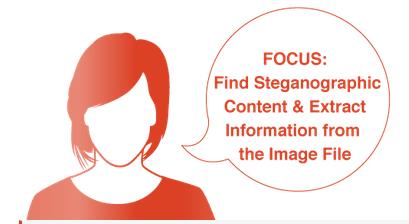
\includegraphics[width=0.85\textwidth]{../../images/python/page_010_img_01.jpeg}

\end{document}
